\section{LTasks}\label{section-ltasks}
To continue the naming scheme of iTasks and mTasks, the proof of concept implementation in this thesis is called LTasks. This section goes into the details of the LTasks library and shows that it is indeed a correct implementation of TOP. To further show that the proof of concept is indeed complete for TOP, chapter \ref{comparison} contains a case study comparison of the breakfast example, while appendix \ref{appendix} contains full examples in both LTasks and iTasks.

\subsection{Task combinators}
While iTasks provides a lot of combinators, we do not need that for a proof of concept so LTasks includes only the essential combinators and some convenience wrappers around them. Here is the list, along with their operators in LTasks or their equivalent in iTasks:
\begin{itemize}
    \item \lua{constant} (\clean{return} in iTasks)
    \item \lua{step} (\lua{~} in LTasks, \clean{>>*} in iTasks), \lua{stepStable} (\clean{>>-} in iTasks) and \linebreak \lua{stepButtonStable} (\clean{>>?} in iTasks)
    \item \lua{parallel}, \lua{anyTask}, \lua{parallelAnd} (\lua{&} in LTasks, \clean{-&&-} in iTasks), \lua{parallelOr} (\lua{|} in LTasks, \clean{-||-} in iTasks), \lua{parallelLeft} (\clean{-||} in iTasks) and \lua{parallelRight} (\clean{||-} in iTasks)
    \item \lua{transform} and \lua{transformValue} (\clean{@} in iTasks)
\end{itemize}

These are the most important functions for building a TOP system, as we defined at the start of this chapter.

\subsubsection{Step}
The step combinator in LTasks implements both \clean{OnValue} and \clean{OnAction}. When there are multiple continuations that run on the same action, the UI shows the user a dialog to choose one of the continuations to step to. iTasks does not handle this as well: it displays two buttons with the same name, but chooses the first task regardless of which button is pressed.

In the example in listing \ref{lst:ltasks_step}, this happens when the user inputs ``Madam, I'm Adam''---which is both a palindrome and a greeting. LTasks will prompt the user which continuation to step to while iTasks will always step to the palindrome continuation task.

\begin{figure}[ht]
\centering
\begin{minted}{lua}
editor.editString("") ~ {
    {fn = function(value)
        return isPalindrome(value)
            and editor.viewInformation(value, "palindrome: ")
    end},
    {fn = function(value)
        return isGreeting(value)
            and editor.viewInformation(value, "greeting: ")
    end}
}
\end{minted}
\caption{The step combinator in LTasks, using multiple \clean{OnAction} continuations of the same action. Listing \ref{lst:clean_step_onaction} shows this example in iTasks.}
\label{lst:ltasks_step}
\end{figure}

\subsubsection{Parallel}
The parallel task combinator in LTasks is a simplified version of the one in iTasks, but the most common usage is present: combining tasks into a list of task values. Listing \ref{lst:ltasks_parallel} shows a simple example of this.

\begin{figure}[ht]
\centering
\begin{minted}{lua}
(task.constant "A" & task.constant "B") ~ {{
    fn = function(x) return editor.viewInformation(x) end
}}
\end{minted}
\caption{The parallel combinator in LTasks. The output of this is \lua{{"A", "B"}}. Listing \ref{lst:clean_parallel} shows this example in iTasks.}
\label{lst:ltasks_parallel}
\end{figure}

\subsubsection{Custom operators}
In Clean it is common to define lots of operators. For example, there are eight different operators for variations of the step combinator. Lua does allow for changing the behaviour of the standard operators, but only up to a point. For example, the result of the comparison operators like \lua{<} is always converted to a boolean \cite{luareferencemanual}. Perhaps the most notable library that uses operators with custom behaviour is LPeg\footnote{\url{http://www.inf.puc-rio.br/~roberto/lpeg/}}. It is not so common to redefine the behaviour of the operators in Lua, so LTasks only uses three operators: \lua{~}, \lua{&} and \lua{|}. Using the \lua{..} operator for \lua{step} more resembles the original meaning---concatenation, putting strings after each other. However that operator does not play well with chaining multiple operators because it is right-associative \cite[\S 3.4.8]{luareferencemanual}.

\subsection{Type matching}
Instead of implementing the type matching algorithm defined in section \ref{section-combinators-type-matching}, we just used the Typed\footref{footnote-typed} library to compare types, which is very strict in what it matches. There is a Lua library for matching data structures called Tamale\footnote{\url{https://luarocks.org/modules/luarocks/tamale}}, however it is not made for matching types and is also strict in what it matches, so we do not use it.

\subsection{Editors}
Instead of providing a single function for creating all types of user input editors like iTasks does, we provide one function per editor type: \lua{editNumber}, \lua{editTable} etc. To create a table editor, the programmer has to provide the table editor with the sub-editors. Listing \ref{lst:ltasks_editors_table} shows what this looks like.

Each editor construction function has an optional parameter for setting the editor's prompt (called a hint in iTasks). This is done to keep the proof-of-concept simple: iTasks uses a \clean{tune} combinator (with \clean{<<@} operator) which can do a lot more, but that is not important for TOP.

\begin{figure}[ht]
\centering
\begin{minted}{lua}
local dateEditor = editor.editTable {
    year = editor.editNumber(),
    month = editor.editString(),
    day = editor.editNumber(),
}
\end{minted}
\caption{Creating a table editor with three sub-editors for \lua{year}, \lua{month} and \lua{day} (adapted from the date example in appendix \ref{appendix-dates}).}
\label{lst:ltasks_editors_table}
\end{figure}

\subsection{User Interface with LTUI}
For simplicity with working with LTUI, we decided to only ever have one UI element of a type at once. Instead of creating a new element every time, the old one is re-used, displayed, and hidden when no longer needed. These re-used elements are defined and created once in \lua{ltuiApp.lua}.
The module \lua{ltuiElements.lua} provides functions that use these reusable elements and set the contents like the task name or the current value.
\lua{ltuiEditor.lua} is the module that then converts these editors into tasks so they can be used with TOP. This module provides the same functions with the same parameters as \lua{terminalEditor.lua}, which provides editors that use standard I/O as a command-line interface instead of a textual UI. Figure \ref{fig:comparison_ltask_ui} shows the textual user interface in action.

% \begin{figure}
%     \centering
%     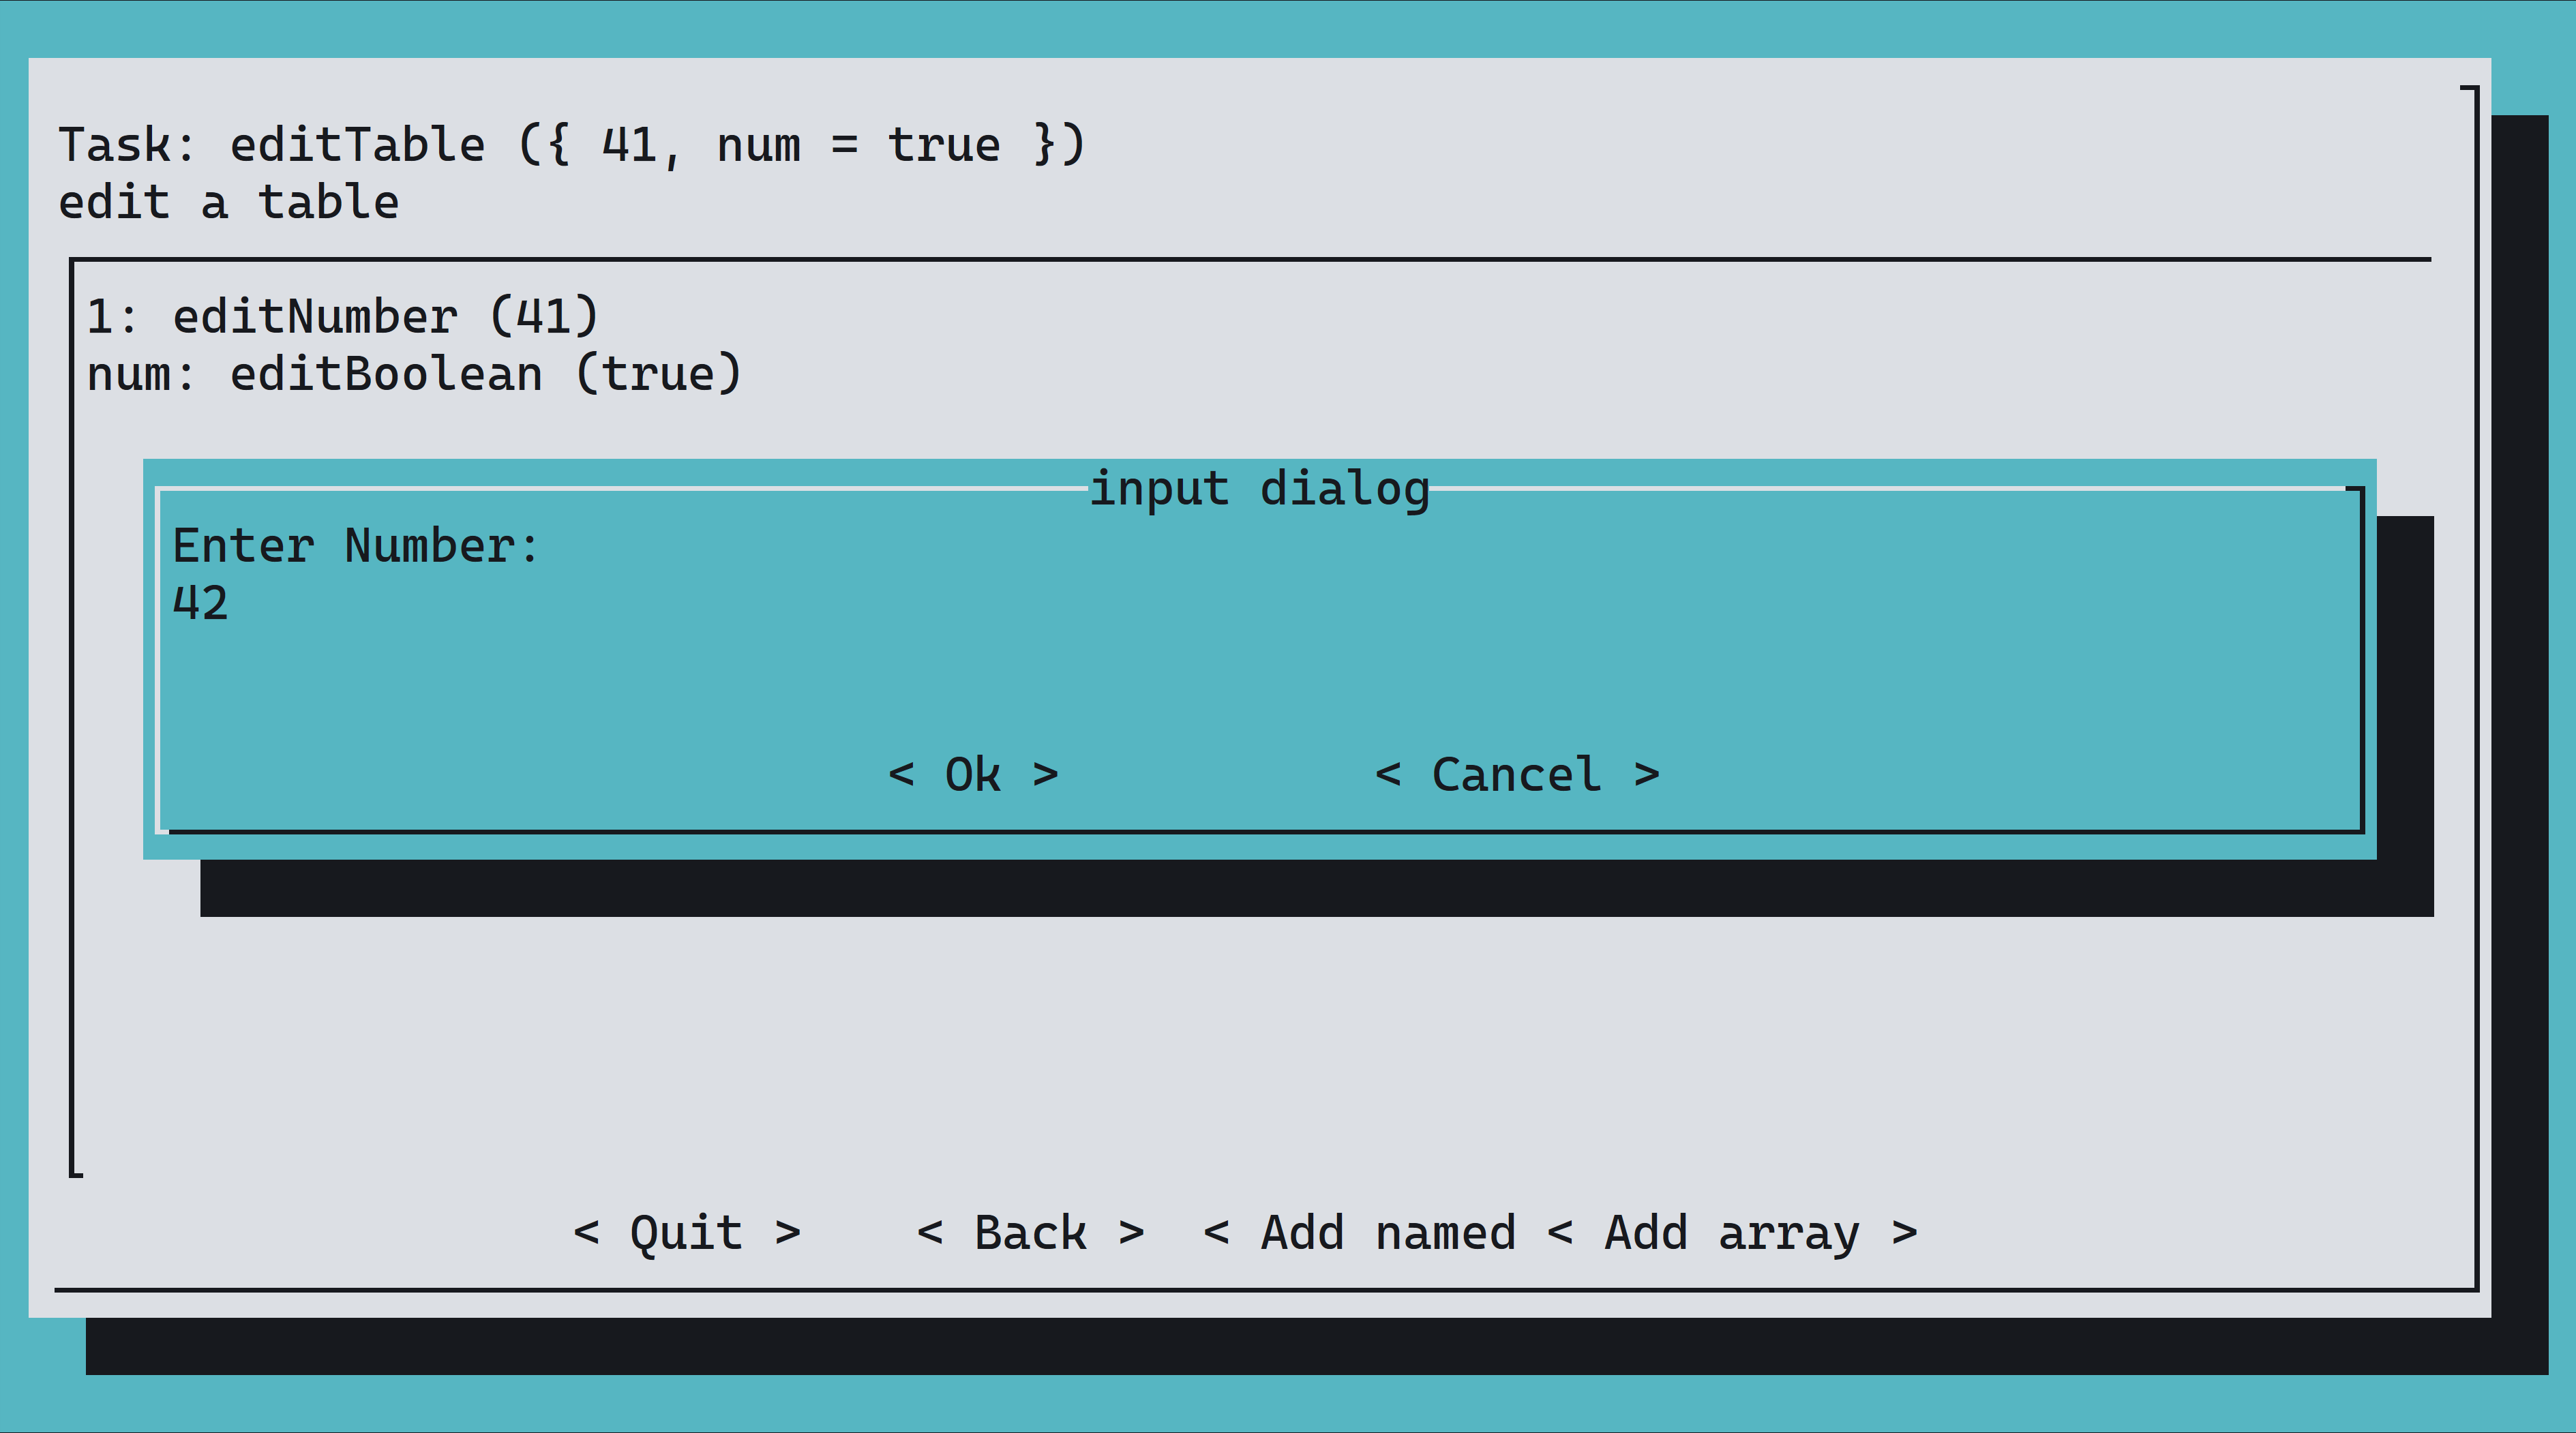
\includegraphics[width=0.8\textwidth]{img/screenshot-ltui.png}
%     \caption{The textual UI showing a table editor in the background with a number input dialog in the foreground.}
%     \label{fig:ltasks_ui}
% \end{figure}
